\section{Introduction}

Modern distributed cloud applications rely heavily on the \emph{partition/aggregate} design pattern, in which an application is broken in into hierarchical layers and time-sensitive requests at higher layers are divided and delegated to workers in the lower layers. Workers perform some component of a task and return a result to an aggregator, which is combined with results from other workers and passed back up through the hierarchy. A problem arises when workers simultaneously report results back to an aggregator, since this traffic must pass through a shared bottleneck, which results in high queueing delays for time-sensitive traffic. 

% why is this an issue? Discuss incast, partition/aggregate pattern, traffic characterization

\section{Improving TCP for Datacenters}

\subsection{Incast TCP}

\subsection{Multipath TCP}

\subsection{TCP BBR}

\subsection{Data Center TCP}

Data center TCP (DCTCP) attempts to address the problem of latency in partition/aggregate traffic by reducing queue length without affecting throughput for large TCP flows.

\section{Reproducing DCTCP Results}

\subsubsection{Methods}

Selected results from \cite{alizadeh_data_2010} were reproduced using the Mininet network emulator running on Ubuntu 12.04 with a patched version of the 3.2.18 Linux kernel patched to add in support for DCTCP. A custom utility was modified from the Mininet utilities repository to monitor queue length, and another utility was created to monitor bandwidth. 

\subsubsection{Results}

\begin{figure}
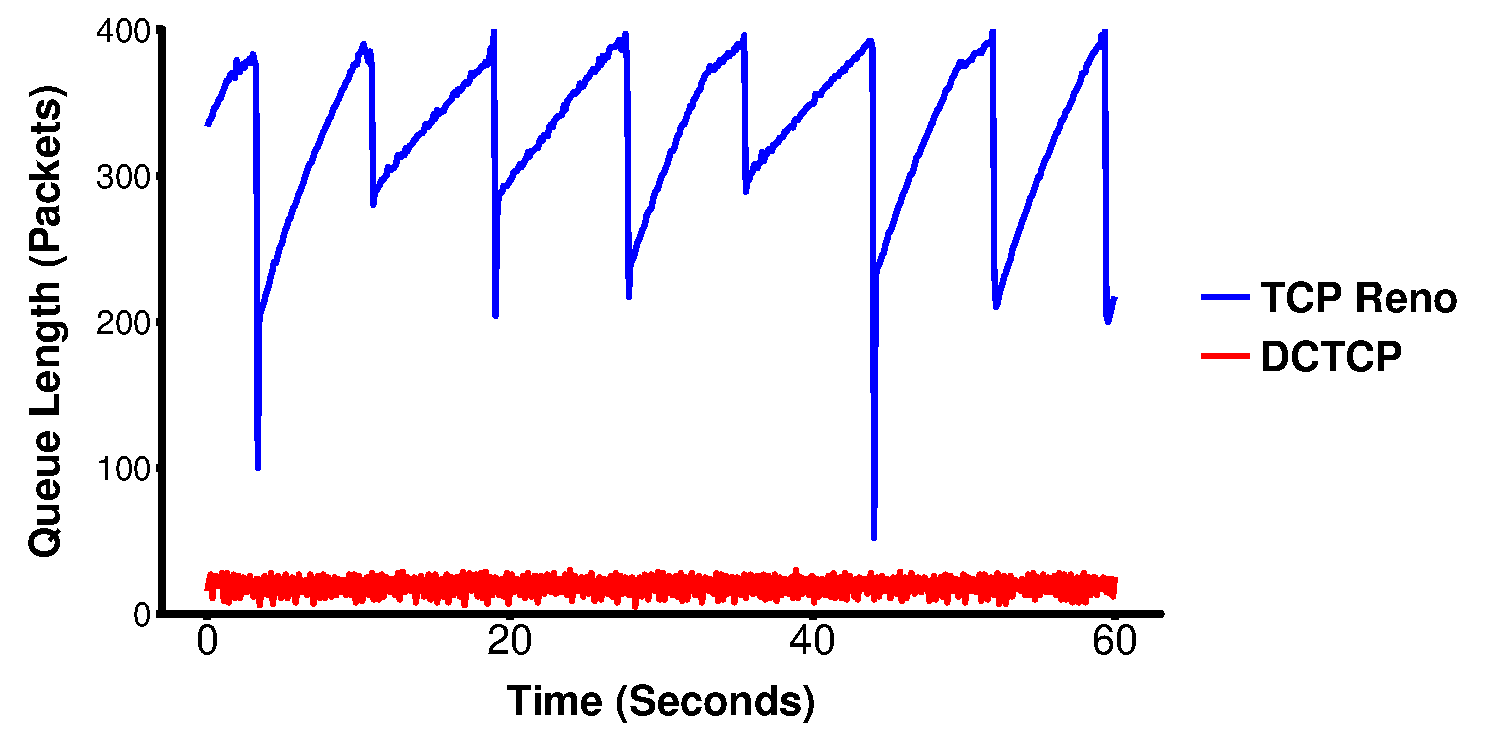
\includegraphics[height=1.75in,width=3.5in]{queue_2_flows}
\caption{Comparison of queue length over time between DCTCP and TCP Reno with 2 flows}
\end{figure}

\begin{figure}
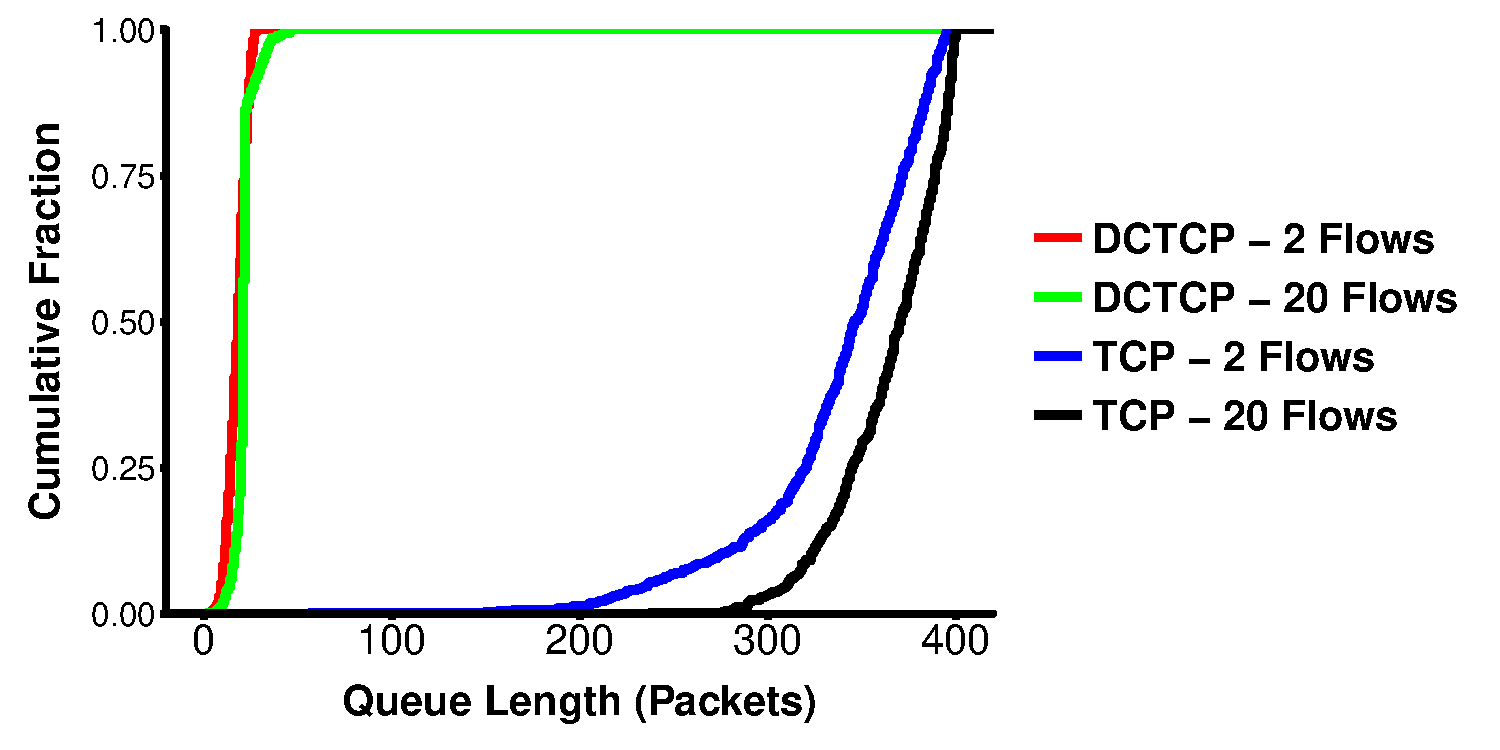
\includegraphics[height=1.75in,width=3.5in]{queue_cdf}
\caption{CDF of queue length for DCTCP and TCP Reno with 2 and 20 flows}
\end{figure}

\begin{figure}
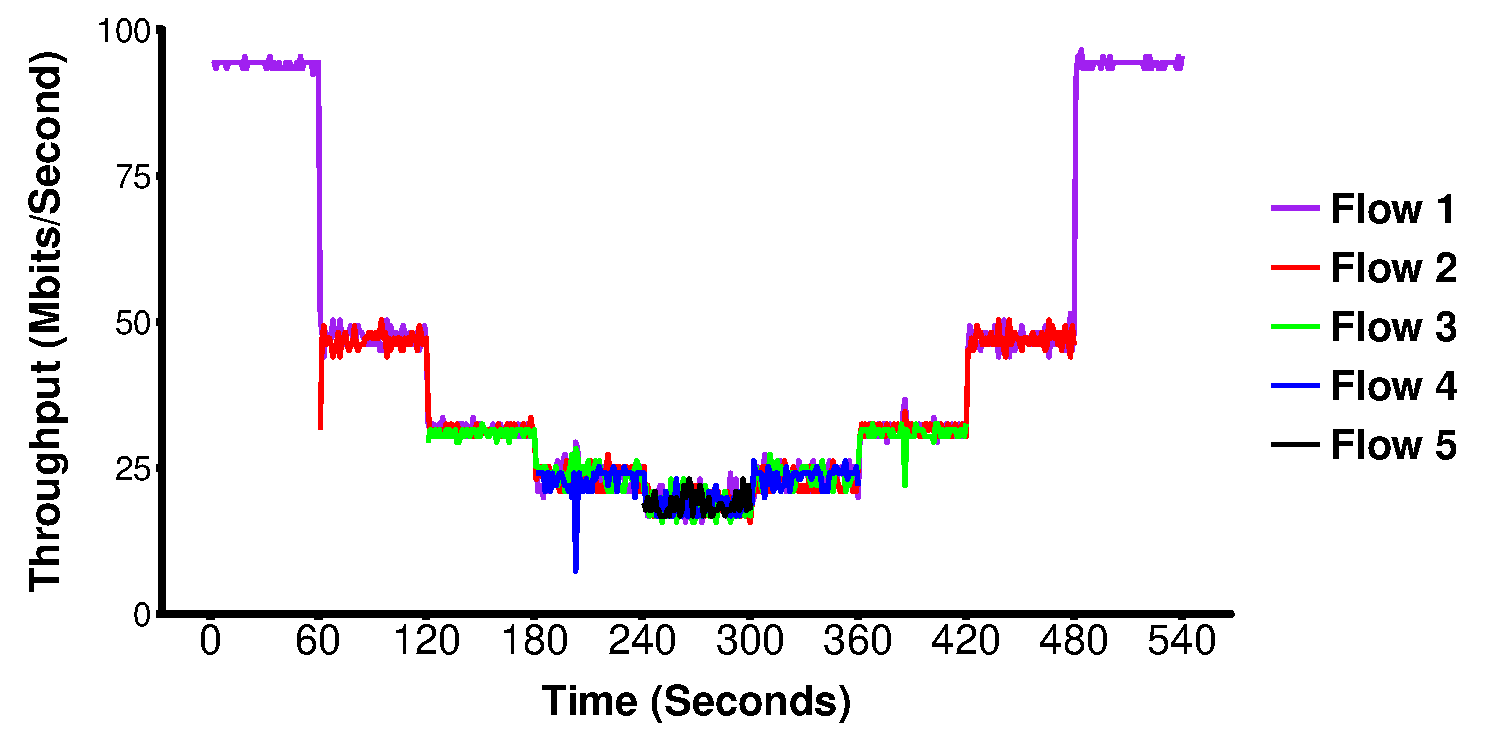
\includegraphics[height=1.75in,width=3.5in]{dctcp_converg}
\caption{Convergence of 5 flows DCTCP}
\end{figure}

\begin{figure}
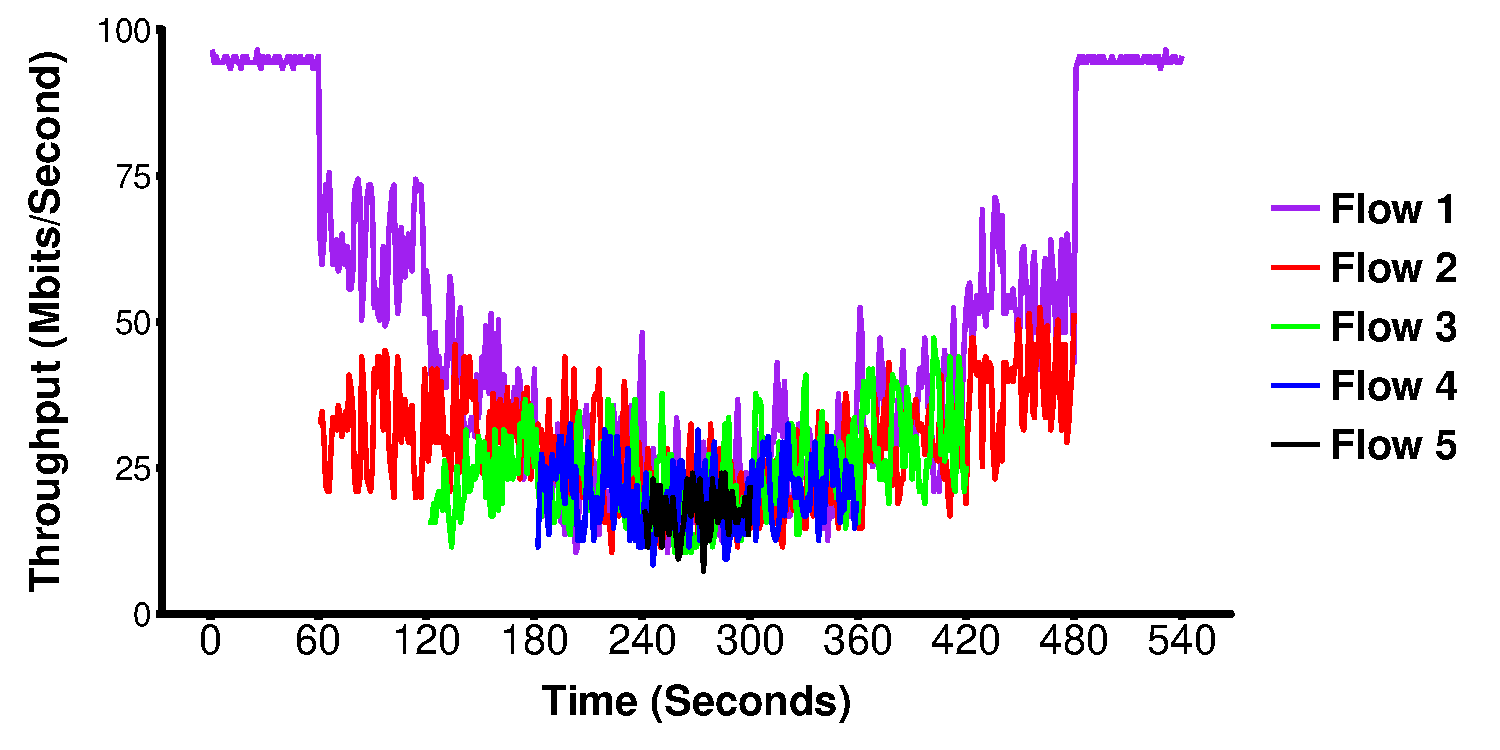
\includegraphics[height=1.75in,width=3.5in]{reno_converg}
\caption{Convergence of 5 flows TCP Reno}
\end{figure}

\begin{figure}
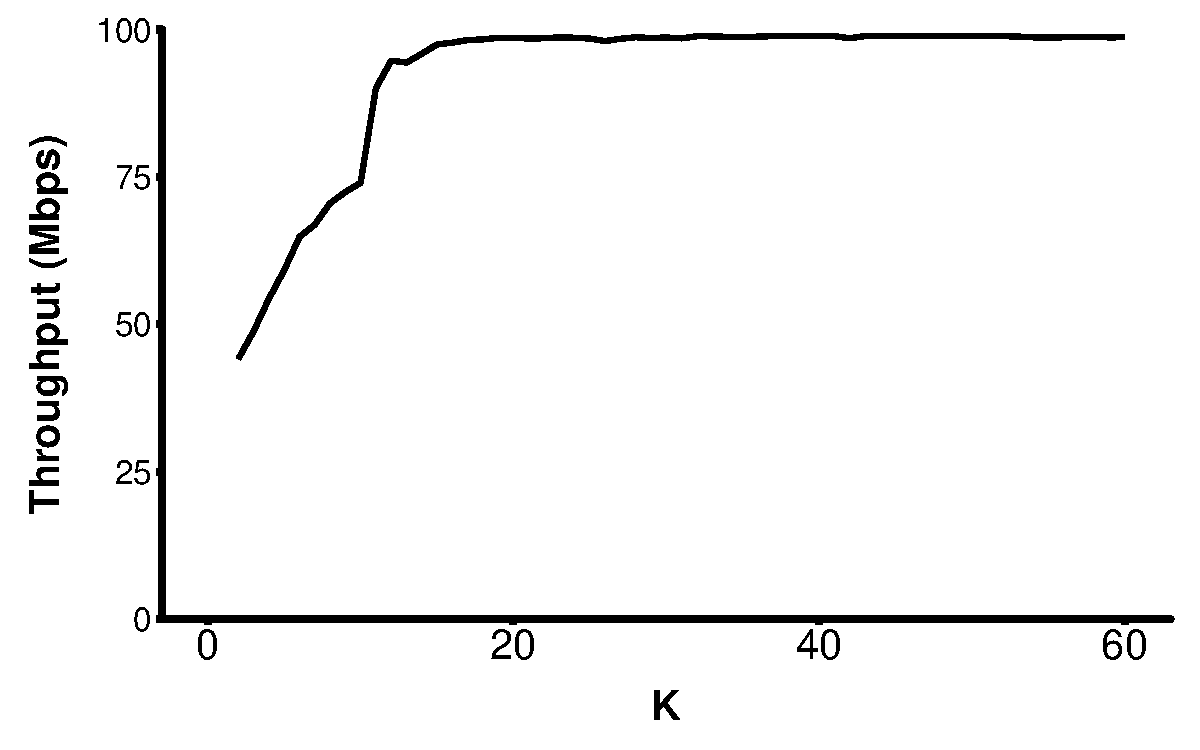
\includegraphics[height=2in,width=3in]{k_throughput}
\caption{DCTCP throughput for varying values of K}
\end{figure}

\subsubsection{Discussion}

\subsubsection{Limitations}

\section{Conclusions}

